\documentclass[a4paper, 11pt]{article}   %设置字号11pt以及A4页面
\usepackage{CJK}               %引入CJK宏包
\usepackage{multirow}
\usepackage{indentfirst} %引入首行缩进宏包
\usepackage{fancyhdr} %页眉页脚宏包
\usepackage{graphicx}
\usepackage{subfigure}
\usepackage{float}
\usepackage{geometry}
\usepackage{graphicx, subfig}
\usepackage{fancyhdr}
\usepackage{setspace}%使用间距宏包
\usepackage{amsmath} 
\usepackage{amssymb} 


\geometry{left=3.1cm, right = 3.1cm, bottom = 3.5cm}       %设置页边距
\setlength{\parindent}{2em} %设置首行缩进两字节

\begin{document}               %begin与end成对出现
\begin{CJK}{UTF8}{gbsn}        %应用CJK环境

\begin{spacing}{1.15} %%行间距变为1.15
%%%%%%%%%%%%%%%%%%%%%%%%%%%%%%%%%%%%%%%%%%%%%%%
%页眉&页脚
 \pagestyle{fancy}
 \lhead{}                         %题注修改
 \chead{}                         %不需要时设置为{}
 \rhead{\bfseries LATEX模板}       
 \lfoot{}                       
 \cfoot{hweigo}                   %页数 \thepage
 \rfoot{\thepage} 
 \renewcommand{\headrulewidth}{0.4pt}
 \renewcommand{\footrulewidth}{0.4pt}
%%%%%%%%%%%%%%%%%%%%%%%%%%%%%%%%%%%%%%%%%%%%%%%
%标题
\title{\huge LATEX模板 \\ \Large -模板小标题-}  
\author{黄威 516021910249\\  
\small 任课老师:XXX,\small 同组组员:XXX, \small 实验日期:XXX}            
\date{}   %\today
\maketitle                         %插入标题
%%%%%%%%%%%%%%%%%%%%%%%%%%%%%%%%%%%%%%%%%%%%%%%
%摘要
\begin{abstract}
该部分内容是放置摘要信息的。该部分内容是放置摘要信息的。该部分内容是放置摘要信息的。该部分内容是放置摘要信息的。该部分内容是放置摘要信息的。
\end{abstract}

%%%%%%%%%%%%%%%%%%%%%%%%%%%%%%%%%%%%%%%%%%%%%%%
%目录
\renewcommand{\contentsname}{目录} %将content改为目录
\tableofcontents                  %插入目录
\newpage
%%%%%%%%%%%%%%%%%%%%%%%%%%%%%%%%%%%%%%%%%%%%%%%
%该语句将图片下标 figure 该为 图
\captionsetup[figure]{labelfont={bf},name={图},labelsep=period}
%%%%%%%%%%%%%%%%%%%%%%%%%%%%%%%%%%%%%%%%%%%%%%%
%该语句将图片标号按章节标注
%注:图标小标仍为总号数,未解决
%\renewcommand {\thefigure} {\thesubsection{}.\arabic{figure}}
%%%%%%%%%%%%%%%%%%%%%%%%%%%%%%%%%%%%%%%%%%%%%%%


\section{Latex模板}


\subsection{正文}
\label{sec:fastguide}
这款移动云台机器人主要针对的是工作在复杂路况环境中的科研人员和相关从业人员,例如抢险救灾的消防员、维修管道的维修工人、地质勘探的科研工作者等等,从事着较为危险的工作,在实际开展工作中面对着难以预料的环境,受限于现有的勘探机器人缺乏强大的越障能力,经常会出现工作失灵的情况,于是工作人员亲自去勘探也就最为常见。\par
~\\                                      %空行
空行\par
                                         %换行符
\textbf{加粗与换行}

\subsection{分点}
\begin{itemize}
\item 没有出色的代替人力的机器人完成相关的工作。咬牙进入危险环境的从业人员极为常见。
\item 现有的移动平台的驱动方式往往只有一种,单一的足式很难保证适应各类环境,亟待整合多种足式运动优势的机器人出现。
\end{itemize}

\subsection{subsubsection}
\label{sec:features}
基于此,我们需要设计的一款移动云台机器人应当具有如下的特点:

\subsubsection{平稳性}
\label{sec:requirements}
移动的云台作为勘探仪器的载体,必须要保证移动时的平稳性,避免因为剧烈震动导致精密仪器的损坏,否则从业人员也不放心安装精密仪器在机器人上,考虑到实际需求才能争取这些特征人群的认可

\subsubsection{平地行驶}
\label{sec:format}
不仅要能够实现越障功能,移动平台机器人在较为平坦的路面上,具有出色的行走能力同样重要。速度太慢而被抛弃的机器人并不在少数。


\newpage                                    %新建一页

%%%%%%%%%%%%%%%%%%%%%%%%%%%%%%%%%%%%%%%%%%%
\section{图片插入}
\subsection{单张图片 - figure}

\begin{figure}[H]
\centering
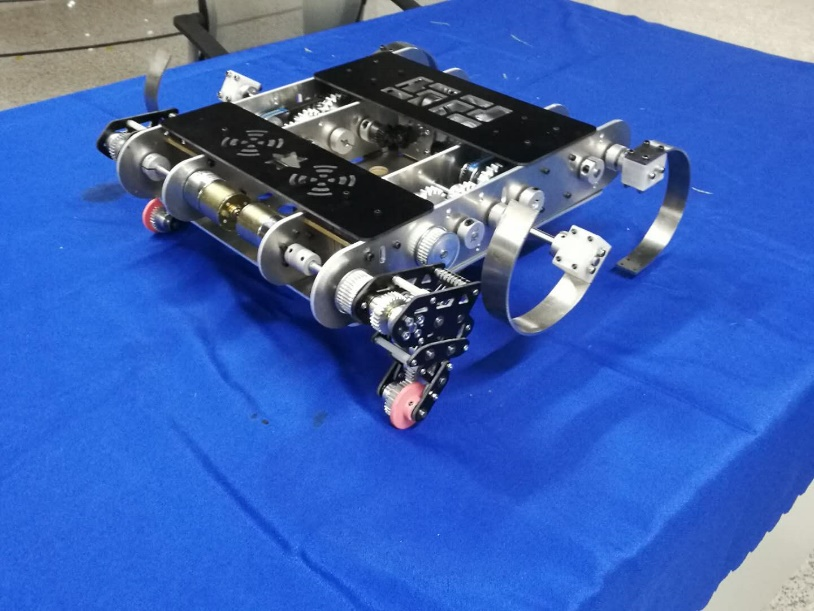
\includegraphics[width=.8\textwidth]{chap2//fig1.jpg}
\caption{主体部分-实物搭建图}
\end{figure}

\begin{figure}[H]
\centering
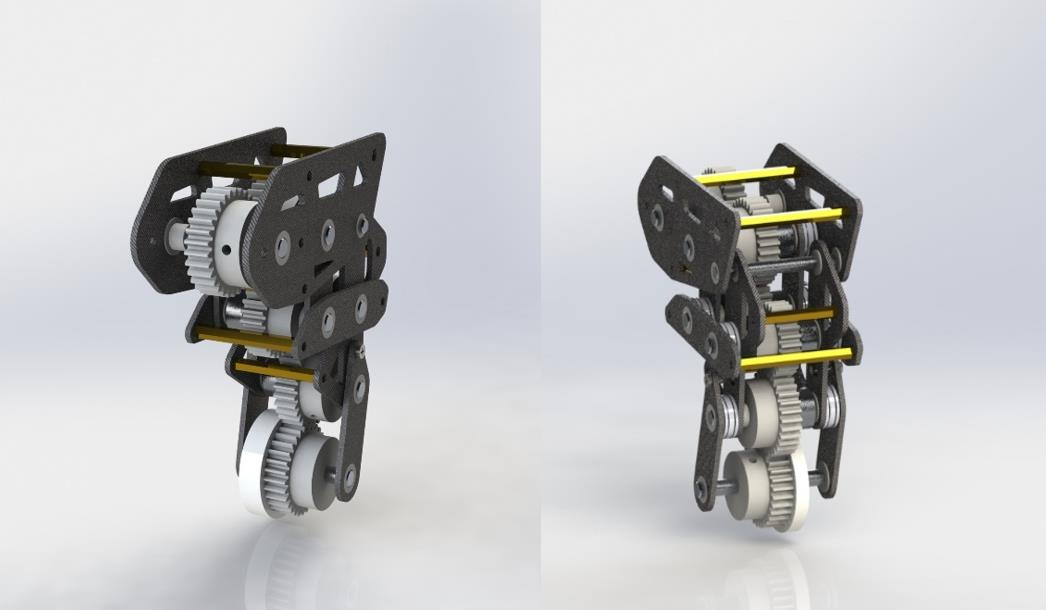
\includegraphics[width=.8\textwidth]{chap2//figa.jpg}
\caption{齿轮系驱动前足-模型渲染图}
\end{figure}

%%%%%%%%%%%%%%%%%%%%%%%%%%%%%%%%%%%%%%%%%%%
\subsection{多张图片 - subfigure}

\begin{figure}[H]
%\centering
\subfigure[框架爆炸图]{
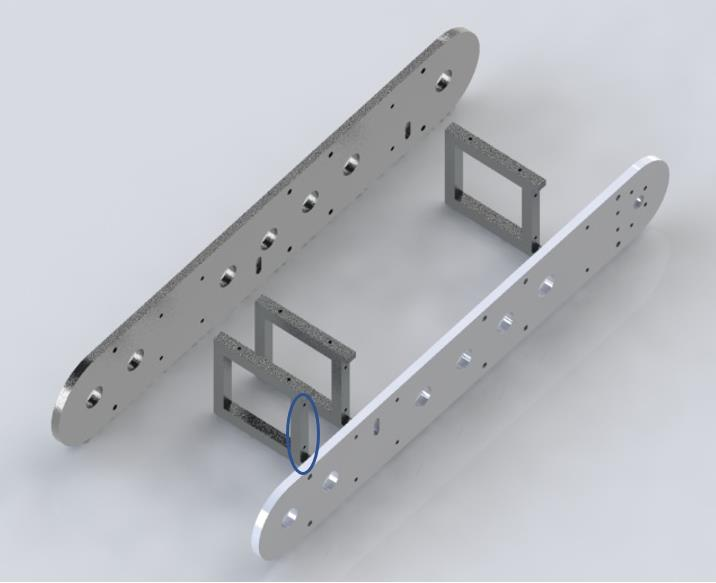
\includegraphics[width=.45\textwidth]{chap2//fig3.jpg}
%\caption{fig1}
}
\quad
\subfigure[框架整合图]{
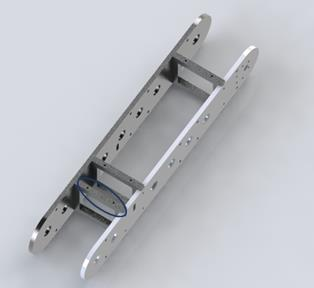
\includegraphics[width=.4\textwidth]{chap2//fig4.jpg}
%\caption{fig1}
}
\quad
\caption{C形足传动框架}
\end{figure}
%%%%%%%%%%%%%%%%%%%%%%%%%%%%%%%%%%%%%%%%%%%
\newpage
\section{公式与表格}
\subsection{公式}

推荐软件:Mathpix Snipping Tool, 截图生成代码。\par
$$K仪\varepsilon仪 = \frac { \Delta R _ { 1 } } { R _ { 1 } } - \frac { \Delta R _ { 2 } } { R _ { 2 } } + \frac { \Delta R _ { 4 } } { R _ { 4 } } - \frac { \Delta R _ { 3 } } { R _ { 3 } } \\ =  \mathrm { K } \varepsilon _ { 1 } - \mathrm { K } \varepsilon _ { 2 } + \mathrm { K } \varepsilon _ { 4 } - \mathrm { K } \varepsilon _ { 3 }$$

$$d_{safe} = \frac{v_{back}^2-v_{front}^2}{2a}$$
式中:\\
k - 仪器灵敏系数指示值\\
$\varepsilon$ - 仪器读数$\mu\varepsilon$\\
K - 电阻应变片的灵敏系数\\

分段函数两种表示方法,使用宏包amsmath。
$$smooth_{L_{1}}(x)=\begin{cases}0.5x^{2}, &\left |x \right |\leq 1 \cr \left |x \right|-0.5, &otherwise\end{cases}$$

大于等于语句$\backslash geq $,小于等于语句$\backslash leq $。

$$
d_{safe}=
\begin{cases}
d_{follow}+d_{length}, &v_{front}\geq v_{back} 
\cr 
d_{follow}+d_{length}+d_{break}, &v_{back}>v_{front}
\end{cases}
$$

\begin{equation}
f(x)=\left\{
\begin{aligned}
x & = & \cos(t) \\
y & = & \sin(t) \\
z & = & \frac xy
\end{aligned}
\right.
\end{equation}

%%%%%%%%%%%%%%%%%%%%%%%%%%%%%%%%%%%%%%%%%%%
\subsection{表格}
~\par
不建议使使用,过于复杂。\par
解决方案:1)excel截图;2)自动生成表格代码(在线or编译器自带)。
\begin{table}[!htbp]
\centering
\caption{R1R7组成半桥}
\begin{tabular}{|c|c|c|c|c|} % 通过添加 | 来表示是否需要绘制竖线
\hline %绘制横线
载荷N&初始值&5&10&15\\
\hline
仪器读数$\varepsilon $\begin{tiny}仪\end{tiny}&0.81&28.36&54.99&81.33\\
\hline
\end{tabular}
\end{table}


\begin{table}[!htbp]
\centering
\caption{R1R2R3R4组成全桥}
\begin{tabular}{|c|c|c|c|c|c|}
\hline
\multicolumn{2}{|c|}{载荷N}&初始值&5&10&15\\
\hline
\multirow{2}*{仪器读数$\varepsilon $\begin{tiny}仪\end{tiny}}&临界&-0.30&0.77&2.20&4.01\\
\cline{2-6}
&对接&-4.64&99.34&203.01&306.52\\
\hline
\end{tabular}
\end{table}


\newpage
\section{示例:电控部分设计}
\subsection{总体概述}
\subsubsection{流程图}
 \begin{figure}[H]
\centering
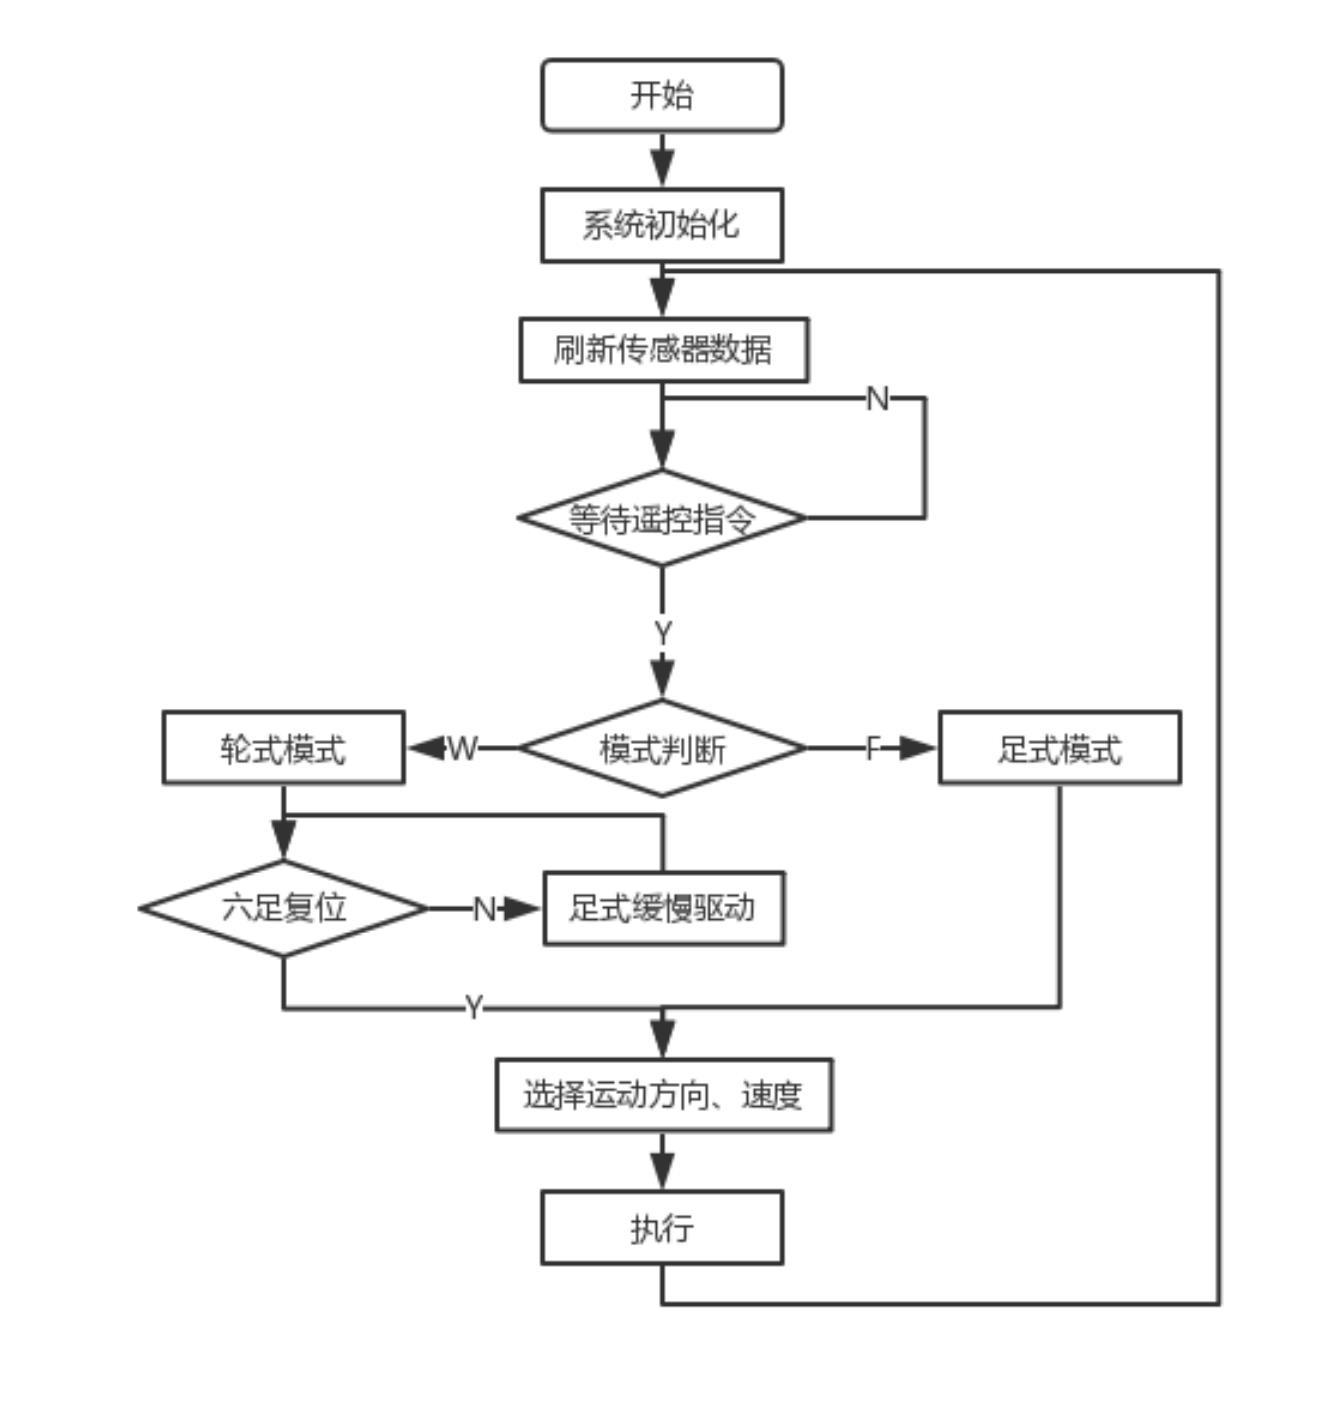
\includegraphics[width=.8\textwidth]{chap5//fig1.jpg}
\caption{控制流程图}
\end{figure}
\subsubsection{功能简介}
\begin{itemize}
\item 足式驱动
\end{itemize}\par
初始化:以两侧轮足平行的上电位置为基准,驱动其中之一侧,使之相差180°;\par
运行:同向同速驱动两侧轮足前进,反向同速驱动两侧旋转。
\begin{itemize}
\item 轮式驱动
\end{itemize}\par
初始化:驱动两侧轮足,使两侧前轮同时处于最低点;\par
运行:同向同速转动前轮前进,差速驱动转弯。

\begin{itemize}
\item 遥控部分
\end{itemize}\par
右上拨杆最上为轮式模式,此时左上拨杆控制高速、低速和停止,右侧摇杆上下推动控制前进后退,左右推动进行转弯;最下为足式模式,此时右侧摇杆上下推动控制前进后退,仅在无前后运动速度的情况下左右推动进行原地旋转控制;中间为停止状态,对任意输入不响应。
\subsubsection{电子器件}
 \begin{figure}[H]
\centering
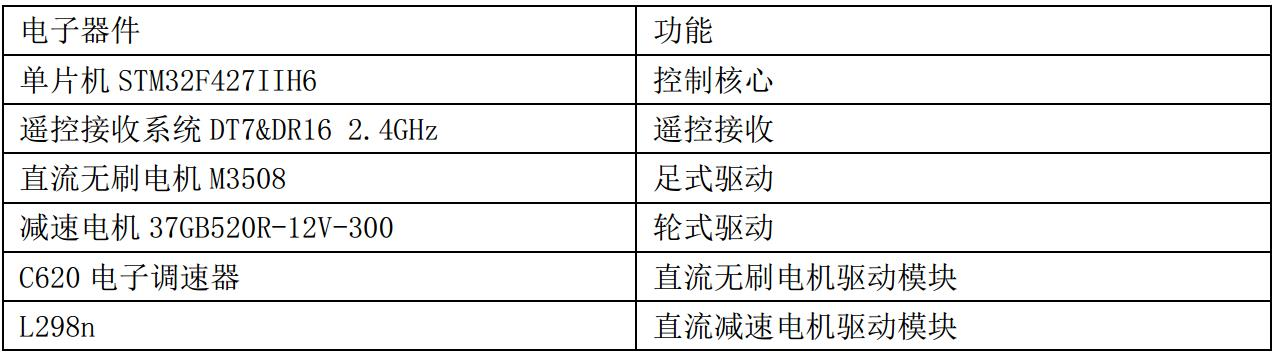
\includegraphics[width=.9\textwidth]{chap5//fig2.jpg}
\caption{电子器件清单}
\end{figure}
\subsubsection{操作系统配置}
 \begin{figure}[H]
\centering
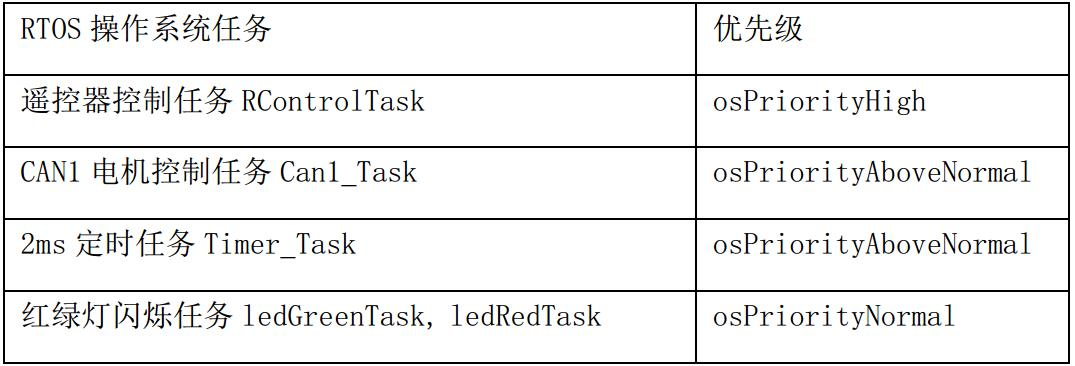
\includegraphics[width=.77\textwidth]{chap5//fig3.jpg}
\caption{操作系统任务及其优先级}
\end{figure}

\subsection{硬件结构}
\subsubsection{硬件结构图}
 \begin{figure}[H]
\centering
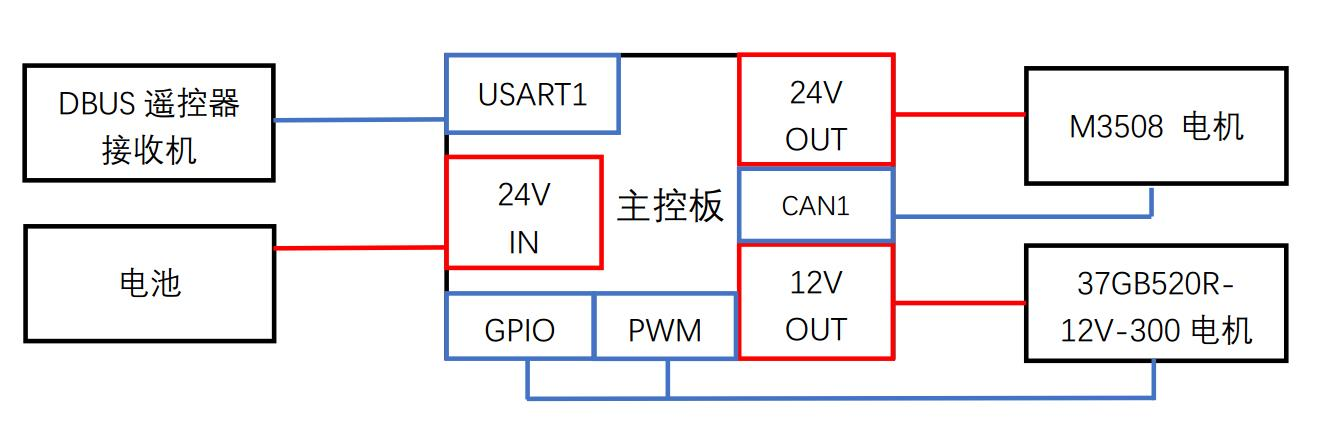
\includegraphics[width=.95\textwidth]{chap5//fig4.jpg}
\caption{硬件结构框图}
\end{figure}
\subsubsection{主控板介绍}
该开发板主控芯片为STM32F427IIH6芯片,通过24v直流电源供电,板载可控电源输出,有丰富的扩展接口和通信接口,可以充分满足控制需求。在本项目中,用到了看门狗、定时中断,串口通信、CAN通信,GPIO、PWM接口。
 \begin{figure}[H]
\centering
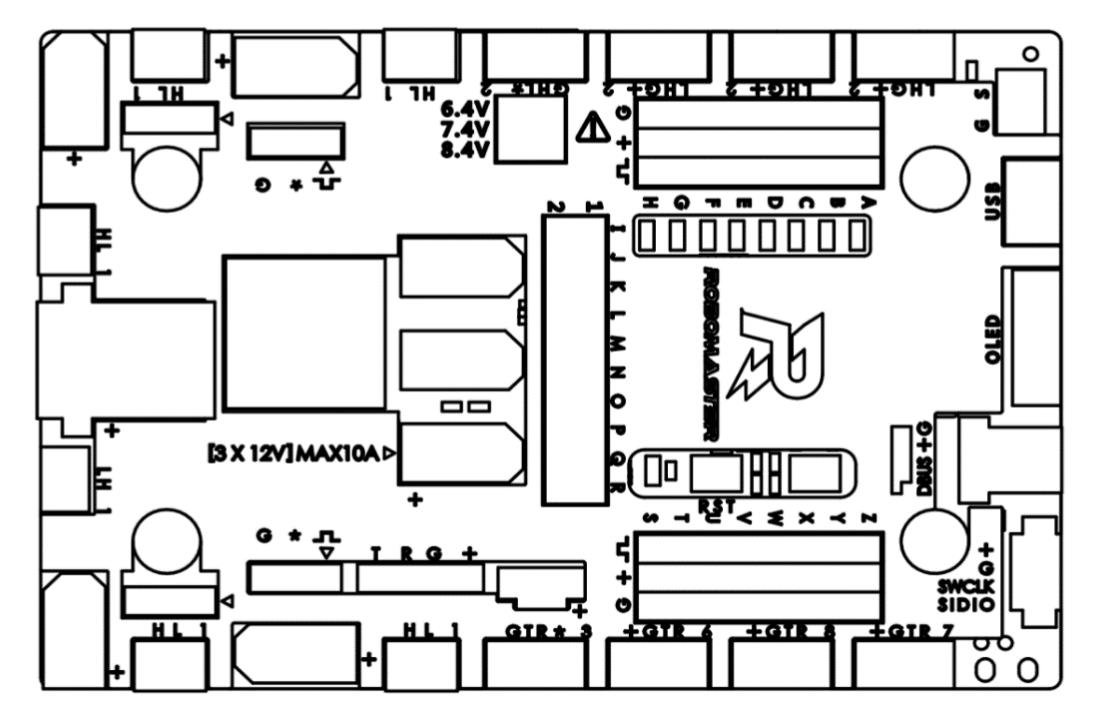
\includegraphics[width=.8\textwidth]{chap5//fig5.jpg}
\caption{主控开发板}
\end{figure}
\subsubsection{动力输出介绍}
M3508无刷直流电机工作电压为24v,最高功率可达220w,最大扭矩5N*m,有感FOC控制在任何转速下都能提供稳定的扭矩,让机器人在快速响应的同时保持平稳的动力。带有编码器,配合C620电调使用,可以得到角度、速度、转矩、温度等参数,通过CAN总线控制,高效方便。该电机可自动感应高温、断线等异常并报警,同时反馈故障,使用安全。
37GB520R-12V-300直流减速电机工作电压为12v,额定力矩2.25kg*cm,通过PWM控制,可实现一定范围内的调速,但占空比直接影响输出电压,过低会使电机无法工作。
\subsection{控制系统}
\subsubsection{程序框架}
 \begin{figure}[H]
\centering
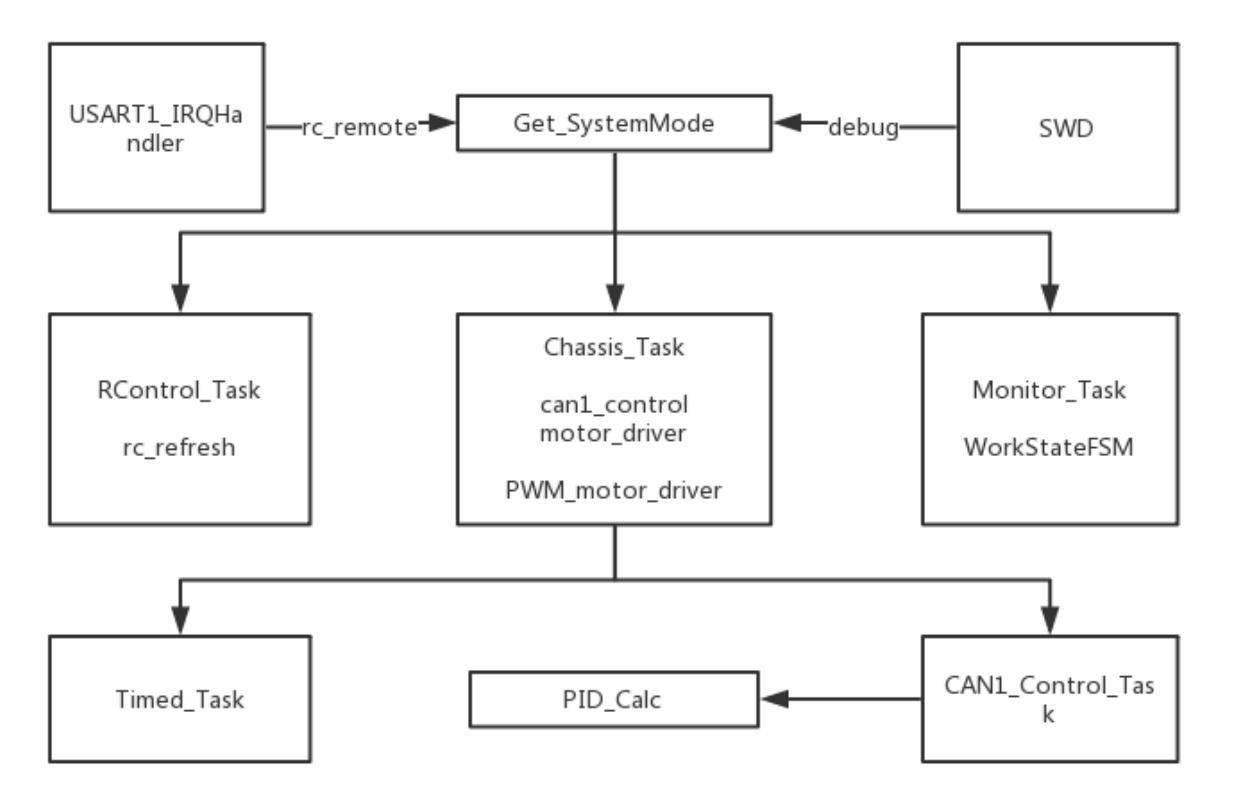
\includegraphics[width=.8\textwidth]{chap5//fig6.jpg}
\caption{程序框图}
\end{figure}
\subsubsection{指令层}
指令层为程序的顶层,该层又分为两部分:遥控器数据读取、整车运行状态机。以遥控器串口中断作为外部输入,是人机交互的接口部分,为了实现人对该六足机器人的控制,该中断为第一优先级,在任何时刻第一时间响应人的指令。\par
整车运行状态监测在定时器中断中进行,包括控制模式切换(足式运行模式、轮式运行模式、以及预留的自动模式)、运行状况状态机(开机启动初始化、电机堵转等应急反应、干扰或潜在bug的异常抛出),使整个控制条理清楚,为进一步开发预留了合理的空间。另外,该程序添加了IWG(看门狗复位),在意外情况下紧急重启,不会发生失控状况。
\subsubsection{控制层}
中间层为控制层,包括足式运行控制、轮式运行控制、红绿状态指示灯三个部分,控制层接收指令层的命令和处理驱动层反馈的数据。\par
对足式驱动电机采用经典的PID控制,主控板与电子调速器之间通过CAN总线通信,主控读取编码器值并解算得到角度、速度,以目标值与实际值之差为输入量,通过双闭环PID算法得到电流作为输出量即控制量,发出电流指令。对轮式驱动电机采用IO控制转向及锁死、PWM控制速度,设置高速、中速、低速三个档位。红绿状态指示灯按照状态机状态出现不同的闪烁情况。
\subsubsection{驱动层}
驱动层为程序底层,包括串口、定时器、CAN总线、GPIO等外设的初始化与驱动,实现与电子调速器之间的数据收发,串行通讯设备之间的数据收发,PWM波输出等底层驱动。在驱动层和控制层之间学习了骆学长的IOPool中间层进行数据交换,读写完全分离,保证了不会出现误修改问题。
\subsection{当前问题及改进方向}
\subsubsection{当前问题}
单侧轮足的耦合运动设计,使得该六足机器人在足式模式下不能实现差速转弯,否则将打乱两侧轮足相差180°的结构,使平台颠簸,损伤机器人。仅能采用原地旋转的方式进行原地转弯。\par
轮式驱动在前足,故如果同速反向驱动电机,机器人将会绕两前足中心旋转,而不是绕整个平台的中心旋转;由于后轮是单向旋转的普通从动轮,后轮在转动过程中会受到平行于轴的侧向力,引起较大的摩擦。\par
由于编码器是针对转子而言,且减速比为19:1,故如果运行过程中出现异常并重启,机器人将无法找到自己的当前位置,对两侧轮足的相对角度控制造成困难。
\subsubsection{改进方向}
针对以上第二个问题,可以根据尺寸和速度进行运动学解算,在旋转时给两轮进行速度补偿,使之绕平台中心旋转。\par
针对以上第三个问题,可以寻找合适的传感器,并找到合适的安装位置,来实现绝对位置的定位。比如磁电接触开关、触碰开关等。\par
说明,该工程为配套改装足式驱动电机为M3508后的程序,源码为文件“六足-stm32”,改自RoboMaster开源代码。 配套展示用42GA775F-12V-110直流电机的Arduino源码见文件“六足-Arduino”。\par
~\\
附,关键代码:
 \begin{figure}[H]
\centering
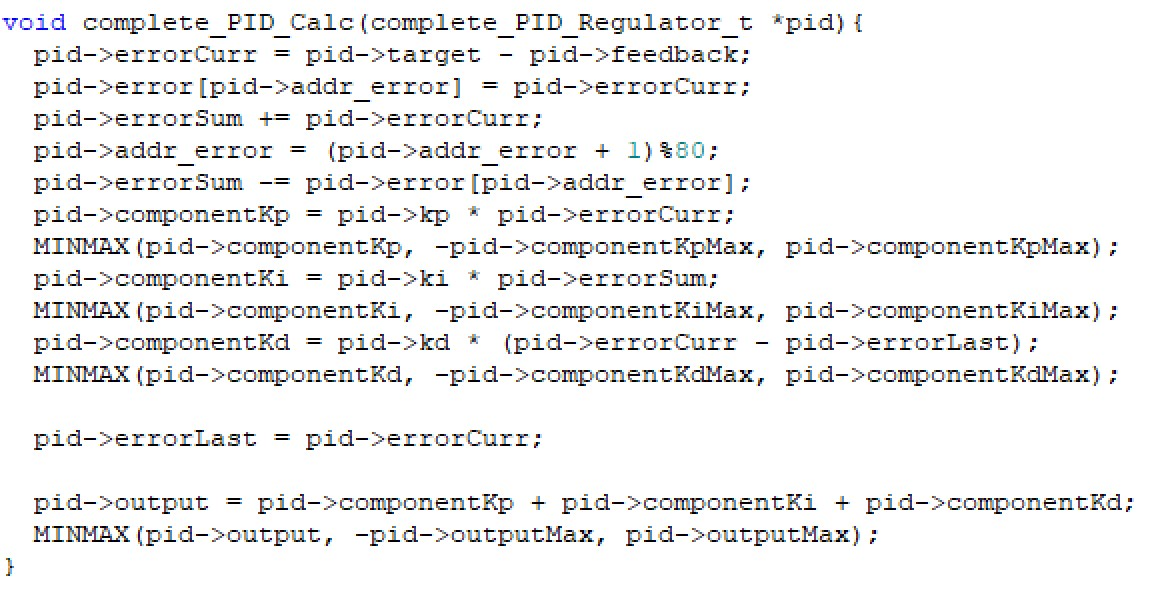
\includegraphics[width=.9\textwidth]{chap5//fig7.jpg}
\caption{双闭环PID角度、速度控制}
\end{figure}
 \begin{figure}[H]
\centering
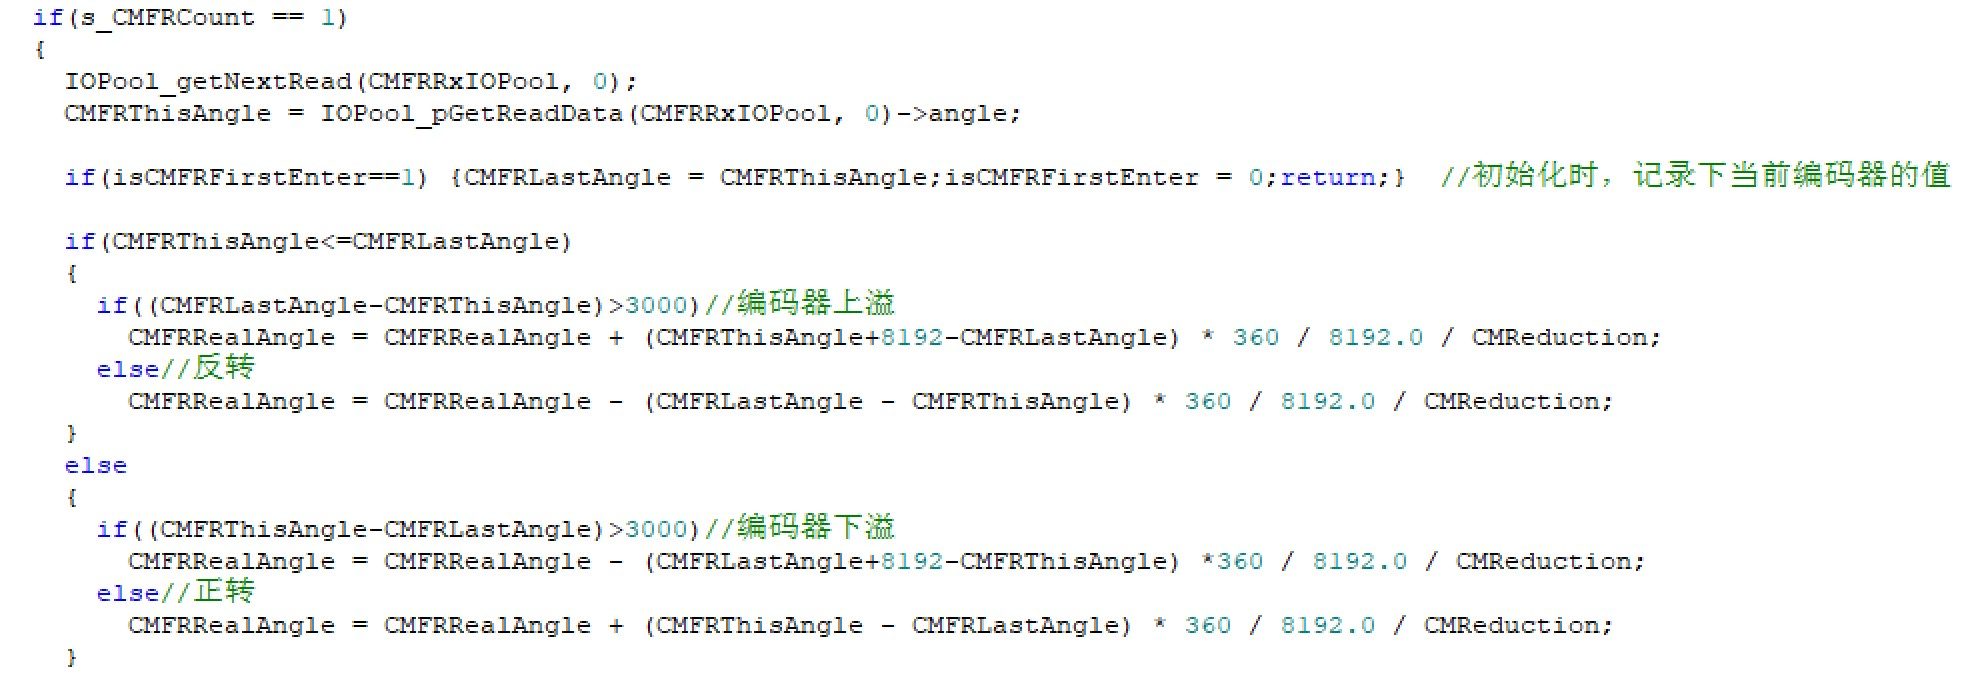
\includegraphics[width=.9\textwidth]{chap5//fig8.jpg}
\caption{编码器溢出算法}
\end{figure}

\end{spacing}
\end{CJK}
\end{document}


 
